\documentclass[10pt,a4paper]{article}

\usepackage[style=numeric, backend=biber]{biblatex}
\usepackage[utf8]{inputenc}
\usepackage[english, catalan]{babel}
\usepackage[pdftex]{graphicx}
\usepackage[margin=1.5in]{geometry}
\usepackage[style=english]{csquotes}
\usepackage[gen]{eurosym}
\usepackage[pdftex, pdfborderstyle={/S/U/W 0}]{hyperref} % this disables the boxes around links

\addbibresource{./bibliography.bib}

\DeclareUnicodeCharacter{20AC}{\euro{}}

\setlength{\parskip}{0.6em}

\author{
    Sánchez Ferreres, Josep\\
}

\title{}

\begin{document}

\begin{titlepage}
\centering{
    \vspace*{5cm}
    \Huge{Comparació de descripcions textuals i formals de models de processos}
    \vspace{0.5cm}\\
    \huge{- Memòria de la fita de seguiment -}\\
    \vspace{3cm}}
    \vfill
    
\flushleft{\large{
    \textbf{Alumne:} Josep Sánchez Ferreres\\
    \textbf{Especialitat:} Computació\\
    \textbf{Director}: Josep Carmona\\
    \textbf{Co-Director:} Lluis Padró\\
    10 de Maig de 2016}}

\thispagestyle{empty}
\end{titlepage}

\tableofcontents

\clearpage

\section{Introducció}

Aquest document correspont al lliurament de la fita de seguiment d'aquest Treball de Fi de Grau. El document parteix de l'informe entregat com a part de la fita inicial, del qual només se n'han modificat els següents apartats:

\begin{itemize}
    \item Apartat \ref{canvis}: Canvis en la metodologia de treball.
    \item Apartat \ref{alternatives}: Anàlisi d'alternatives i decisions.
    \item Apartat \ref{estat}: Estat del projecte en la planificació.
    \item Apartat \ref{integracio}: Integració de coneixements.
    \item Apartat \ref{lleis}: Lleis i regulacions.
\end{itemize}

Cal notar també, que aquest document reflecteix l'estat del projecte a data de 10 de Maig de 2016, i que no s'hi troben reflectits canvis posteriors.


\section{Abast del projecte i contextualització}

\subsection{Context}

Aquesta secció conté una contextualització de l'àmbit d'estudi del projecte. En els primers apartats es fa referència als camps d'estudi que tenen a veure amb aquest i finalment a l'apartat \ref{el_projecte} es defineix quin és el projecte que es durà a terme tot justificant la seva utilitat i públic objectiu.

\subsubsection{Natural Language Processing \& Understanding}

El \emph{Natural Language Processing} (NLP) és un camp en la informàtica que tracta les interaccions entre els ordinadors i el llenguatge natural dels humans. El NLP tracta diversos tipus de problemes a diferents nivells d'abstracció, des dels més purament linguistics com l'anàlisi morfosintàctic d'oracions o determinar la categoria gramatical d'una paraula (\emph{POS-tagging}) fins a la creació de resums automàtica de notícies d'un diari.

Aquells problemes que tenen a veure amb, no només reconèixer i dividir el text sinó que també pretenen entendre el contingut i derivar-ne informació semàntica cauen en el camp del \emph{Natural Language Understanding} (NLU). L'objectiu del NLU és construir representacions semàntiques completes dels textos, de forma que siguin processables, i.e. comprensibles, per a una màquina. Es tracta, doncs, d'un problema IA-complert \cite[][secció 1]{ai_completeness}, ja que els textos estan escrits per a lectors humans i pressuposen sentit comú i coneixements del món: Coses molt difícils d'incloure en un programa.

\subsubsection{Processos de negoci}

En el món corporatiu, a l'hora de descriure com opera una empresa se sol parlar en termes de processos de negoci (\emph{business process}). Un procés de negoci es pot definir, de forma abstracta, com una col·lecció de tasques descrites de forma estructurada i que permeten produir un producte o servei concret. En altres paraules, un procés és la descripció de com es duu a terme una certa operació en una empresa, indicant com es mou la informació a través dels diferents agents implicats i quines tasques es realitzen a cada pas.

És en aquest àmbit que apareix el camp del \emph{Business Process Management} (BPM). El BPM engloba l'estudi i modificació d'aquests processos amb l'enfoc específic de millorar-los optimitzant com, i en quin ordre, es porten a terme les tasques que descriu.

Moltes empreses fan servir BPM tant per documentar com per millorar l'eficiència dels seus processos de negoci, i com a resultat d'això, mantenen grans repositoris d'informació amb aquests processos. És vital, doncs, mantenir aquesta informació actualitzada i coherent, i és en aquest problema on neix la motivació per aquest treball.

\subsubsection{Descripció de processos: Textual i BPMN}

És evident la necessitat de representar d'alguna manera els processos de negoci per tal que els actors implicats puguin entendre'ls així com perquè els encarregats del \emph{business process management} puguin millorar-los.

La primera forma de representar processos que es tractarà en aquest treball, i també la més evident, és la textual. Consiteix en descriure el procés en un document fent servir llenguatge natural. La figura \ref{fig:example_text} mostra un exemple de representació textual d'un procés. Tot i generalment ser la més senzilla d'interpretar \cite{text_with_bpmn} per part de les persones implicades en el procés, el fet que es tracti d'informació no estructurada i la ambiguitat inherent al llenguatge natural dificulten molt el tractament d'aquests processos des de l'enfoc del BPM. És per això que apareix el \emph{business process model and notation} (BPMN). 

El BPMN és un estàndard de representació gràfica de processos de negoci creat per la \emph{Business Process Management Initiative} (BPMI)\footnote{Actualment l'estàndard de BPMN està mantingut per l'\emph{Object Management Group} (OMG).}. La figura \ref{fig:example_bpmn} mostra un exemple d'aquesta notació. 

El BPMN ofereix nombrosos avantatges sobre la representació textual: En primer lloc, permet representar de forma molt més inambigua el contingut, tractant-se d'informació estructurada en forma de diagrama. A més, donada la seva estructura es pot tractar molt més fàcilment amb software; permetent aplicar anàlisi formal per a extreure conclusions globals sobre el comportament dels processos. Finalment, existeixen motors d'execució que a partir d'un BPMN controlen l'execució d'un procés a temps real, permetent a més executar automàticament totes les tasques que puguin ser definides per un \emph{script}. Tot això fa que l'ús del BPMN sigui molt valuós per a una empresa que vulgui automatitzar l'anàlisi i execució dels seus processos.

Els avantatges tecnològics del BPMN respecte a la representació textual són evidents. No obstant això, diferents tipus d'\emph{stakeholders} prefereixen diferents tipus de notació perquè els hi resulta més fàcil d'entendre o perquè no coneixen bé el BPMN.

\begin{figure}
\centering
\begin{minipage}{0.9\textwidth}
\small\emph{{The examination process can be summarised as follows. The process starts
when the female patient is examined by an outpatient physician, who decides
whether she is healthy or needs to undertake an additional examination. In the
former case, the physician fills out the examination form and the patient can
leave. In the latter case, an examination and follow-up treatment order is placed
by the physician who additionally fills out a request form. Beyond information
about the patient, the request form includes details about the examination 
requested and refers to a suitable lab. Furthermore, the outpatient physician
informs the patient about potential risks. If the patient signs an informed consent
and agrees to continue with the procedure, a delegate of the physician
arranges an appointment of the patient with one of the wards. The latter is
then responsible for taking a sample to be analysed in the lab later. Before the
appointment, the required examination and sampling is prepared by a nurse of
the ward based on the information provided by the outpatient section. Then, a
ward physician takes the sample requested. He further sends it to the lab indicated
in the request form and conducts the follow-up treatment of the patient.
After receiving the sample, a physician of the lab validates its state and decides
whether the sample can be used for analysis or whether it is contaminated and
a new sample is required. After the analysis is performed by a medical technical
assistant of the lab, a lab physician validates the results. Finally, a physician
from the outpatient department makes the diagnosis and prescribes the therapy
for the patient.}}
    \end{minipage}
    \caption{Exemple de text que descriu un procés de negoci.}
    \label{fig:example_text}
\end{figure}

\begin{figure}
    \begin{center}
        \makebox[\textwidth]{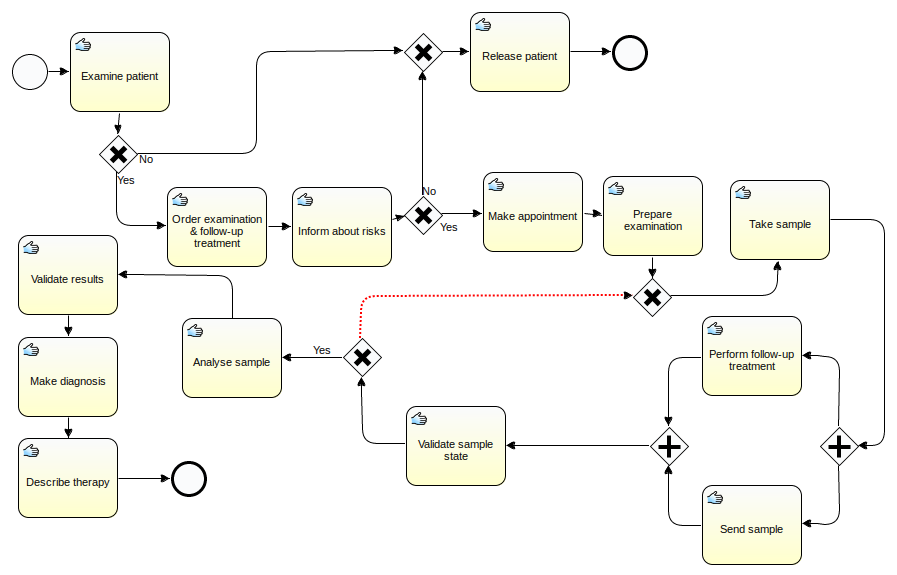
\includegraphics[width=\textwidth]{UlmHospital.png}}
    \end{center}
    %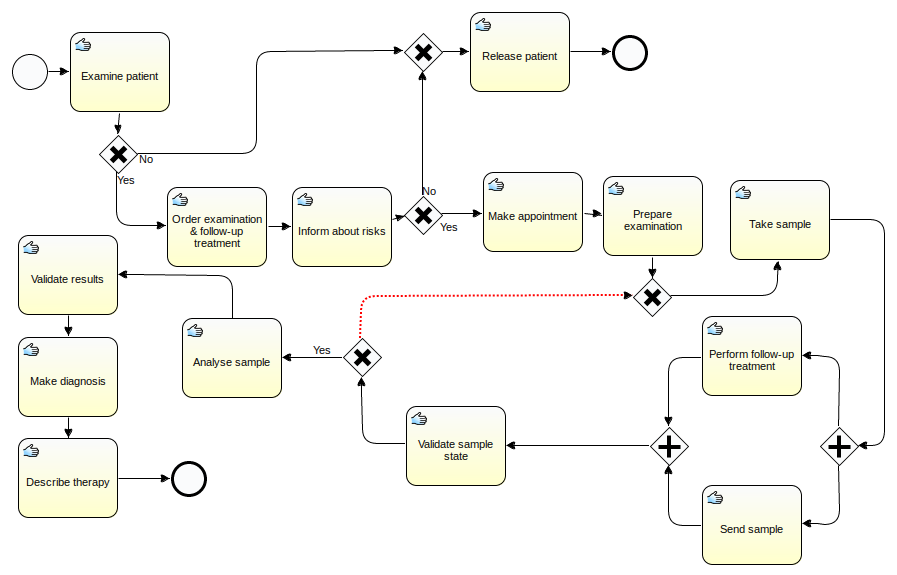
\includegraphics[width=0.9\paperwidth]{UlmHospital.png}
    \caption{Exemple de model BPMN corresponent al text de la figura \ref{fig:example_text}}
    \label{fig:example_bpmn}
\end{figure}

\subsubsection{El projecte}
\label{el_projecte}

Com que no hi ha un clar vencedor entre la representació textual i la notació BPMN a l'hora de representar processos, moltes vegades s'opta per mantenir el procés documentat d'ambdues maneres. Tenint en compte que en una empresa gran s'estan documentant centenars d'aquests processos, mantinguts per diversos grups de persones i utilitzant diferents eines d'edició és molt probable que tard o d'hora es produeixin inconsistències entre la descripció textual i el model BPMN que representen el mateix procés. Aquestes incoherències són una font de problemes en el procés de producció de l'empresa en qüestió, i solucionar-los manualment requereix una inversió en temps i diners.

Donat aquest problema, és evident el gran avantatge d'automatitzar la tasca de comparar el model BPMN amb la corresponent descripció textual, però la dificultat per tractar amb textos no estructurats fa que aquest sigui un terreny molt inexplorat. 

El projecte del qual formo part és una iniciativa que pretén combinar el món del \emph{Natural Language Processing} i el \emph{Business Process Management} amb l'objectiu de la creació d'una eina per assistir l'automatització de tasques relacionades amb el modelat de processos de negoci. Les parts que s'estan desenvolupant actualment en aquest projecte són les següents:

\begin{itemize}
    \item Un traductor de descripcions textuals de processos a models BPMN.
    \item Un traductor de models BPMN a descripcions textuals de processos.
    \item Una eina que permeti trobar inconsistències entre models BPMN i descripcions de processos.
    \item Una eina gràfica que integri totes les funcionalitats esmentades anteriorment en un únic paquet de software.
\end{itemize}

La meva tasca en el projecte, i l'objectiu d'aquest treball, consisteix a implementar l'eina que permeti comparar les dues representacions trobant possibles inconsistències.


\subsection{Estat de l'art}

En aquesta es parla de l'estat de l'art en el problema específic que aquest projecte pretén resoldre. 

\subsubsection{Solucions anteriors}

El problema que tracta aquest projecte, la comparació de models textuals i models de processos en BPMN, és un camp molt inexplorat. Només hi ha un grup \cite{el_paper} que hagi publicat un article proposant una solució a aquest problema. 

La solució que proposa \cite{el_paper} consisteix, igual que aquest projecte, en combinar el BPM amb tècniques de NLP. L'algoritme (veure figura \ref{fig:el_paper_fig}, a grans trets, és el següent:

\begin{enumerate}
    \item Separar el text en frases i el model en tasques.
    \item Analitzar i simplificar el text del model i de les frases amb una eina de NLP\footnote{Concretament l'eina utilitzada és l'\emph{Stanford Parser} \cite{stanford_parser}}.
    \item Computar una \emph{score} de similaritat entre les parelles frase-tasca.
    \item Trobar una assignació òptima que doni la correspondència entre frases del text i tasques del model.
    \item A partir de la informació computada, trobar les inconsistències entre el model i el text.
\end{enumerate}

\begin{figure}[bth]
    \centering
    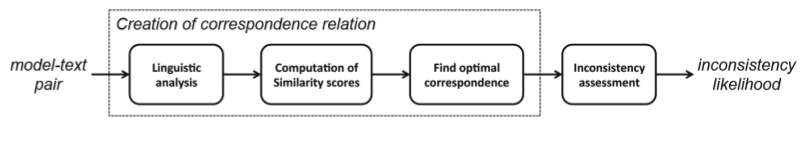
\includegraphics [width=\textwidth]{el_paper_fig.png}
    \caption{Estructura bàsica de la solució proposada en \cite{el_paper}}
    \label{fig:el_paper_fig}
\end{figure}

Centrant-nos en l'apartat d'anàlisi lingüístic, El tractament que es fa a les paraules del text és el següent:

\begin{description}
\item[\textbf{Resolució d'anàfores:}] Els pronoms (\emph{him}, \emph{her}, ...), i alguns determinants (\emph{this}, \emph{that}, ...) del text se substitueixen pel mot al qual fan referència:\\ \emph{him $\rightarrow$ manager}
\item[\textbf{Extracció de clàusules:}] S'eliminen les clàusules secundàries del text, per centrar-se només en les parts de la frase que defineixin una acció del model i eliminar mots que podrien afegir soroll a l'hora de computar similaritats.
\item[\textbf{Sanitització del text:}] S'eliminen les \emph{stopwords}\footnote{Paraules que no aporten significat substancial a la frase, com articles o preposicions.} i les paraules restants se substitueixen per l'arrel del mot:\\ \emph{prepared $\rightarrow$ prepare}

\end{description}

\subsubsection{Limitacions d'estudis anteriors}

Aquest projecte basa la seva estructura general en les idees descrites en \cite{el_paper}. En concret també s'ha modelat el problema com trobar una assignació òptima de frases a tasques.  Cal destacar, de l'estudi esmentat a l'apartat anterior, que l'únic que s'utilitza del model són les frases contingudes en els blocs de les tasques. Tota la informació estructural que proporciona el model s'ignora a l'hora de determinar quina frase del text correspon a cada frase del model. 

Tot i seguir una estructura similar, aquest projecte pretén anar més enllà a l'hora d'extreure informació tant del text com del model, considerant no només informació lèxica sinó també semàntica. Mentre l'algoritme proposat a \cite{el_paper} només tracta les frases com a llistes de paraules aquest projecte tractarà amb informació semàntica a més alt nivell, com qui és el subjecte de l'acció descrita en una frase o quina és aquesta acció. 

\subsection{Formulació del problema}
\label{formulacio}

El problema que es vol resoldre amb aquest projecte es pot resumir en el següent enunciat: 

\begin{displayquote}
Donats un model BPMN i una representació textual d'un procés, determinar si corresponen al mateix procés donant una \emph{score} de similaritat i detectar les possibles incoherències que hi pugui haver entre els dos.
\end{displayquote}

L'objectiu principal del treball és, doncs, la creació de l'algoritme que resol el problema anterior. Més específicament, el treball s'ha dividit en els següents subobjectius:

\begin{enumerate}
    \item Utilitzar tècniques de NLP, fent servir \emph{freeling}\footnote{\emph{Freeling} \cite{freeling} és una eina de software lliure per a \emph{Natural Language Processing} creada pel professor Lluís Padró de la Universitat Politècnica de Catalunya.} des del \emph{Textserver}\footnote{El \emph{Textserver} \cite{textserver} és una plataforma online que proporciona serveis web d'anàlisi linguístic de textos. Fa servir freeling.}, per extreure informació de cada frase de la descripció textual d'un procés.
    \item Explorar models BPMN i analitzar el seu contingut amb tècniques de NLP per tal d'extreure informació de cadascun dels seus elements.
    \item Crear una representació homogènia d'elements del model BPMN i de la descripció textual.
    \item Determinar una mètrica de similaritat per comparar la informació extreta del text i el model.
    \item Determinar una noció de distància entre frases del text i tasques del model.
    \item Utilitzar un algoritme d'optimització o satisfacció de restriccions, utilitzant la informació obtinguda, pugui crear un \emph{mapping} de les frases del text als corresponents elements del model.
    \item Fer servir el \emph{mapping} obtingut del punt anterior per tal de detectar possibles incoherències entre el text i el model.
\end{enumerate}


\subsection{Abast del projecte}

En aquesta secció es fa una descripció extensiva de l'abast i objectius d'aquest projecte. L'apartat \ref{objectiu} parla del producte mínim que es vol aconseguir i possibles ampliacions a aquest. L'apartat \ref{obstacles} parla dels possibles obstacles que han sorgit, o poden sorgir durant el desenvolupament del treball.

\subsubsection{Objectiu}
\label{objectiu}

L'objectiu d'aquest projecte és dissenyar un algoritme que resolgui el problema descrit a la seccio \ref{formulacio}. El procés descrit per aquests objectius es pot visualitzar al diagrama de la figura \ref{fig:estructura_projecte}. De les frases i el model se n'extreuen els \emph{UR}\footnote{Abreviació de \emph{Unified Representation}} (Objectius 1, 2 i 3). A continuació es comparen els \emph{UR} d'un cantó amb els de l'altre, per obtenir tant la matriu de similaritat (Objectiu 4) com la de distància (Objectiu 5). Aquestes matrius passen a ser les dades d'entrada d'un algoritme d'optimització per establir l'assignació òptima\footnote{Cal notar que aquesta assignació no ha de ser necessàriament bijectiva.} (Objectiu 6). Finalment s'utilitza la resposta de l'algoritme per determinar on són els punts d'interès i extreure les incoherències que hi puguin haver (Objectiu 7).

Com a possibles ampliacions al projecte base, s'han plantejat els següents objectius addicionals:

\begin{enumerate}
    \item Estudiar les possibilitats de reduir el problema a un LAP\footnote{\emph{Linear Assignment Problem} \cite{LAP}}, que té solució en temps polinòmic, per determinar una solució inicial per l'algoritme d'optimització.
    \item Experimentar quina és el millor subconjunt d'informació a extreure eliminant possibles causes de soroll al càlcul de similaritat.
    \item Experimentar amb diverses mètriques de similaritat i fer una comparativa per determinar quina s'escau més al domini del problema.
    \item Investigar i experimentar diferents tipus d'algoritmes d'optimització per determinar quin és el més eficient i ofereix solucions de més qualitat al problema objectiu.
\end{enumerate}


\begin{figure}
    \centering
    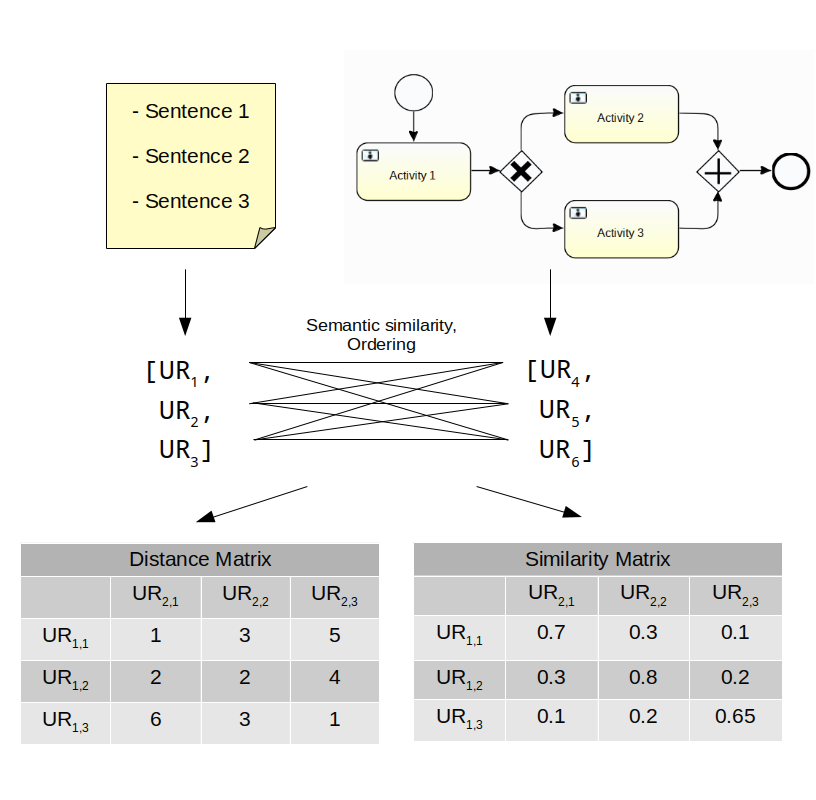
\includegraphics[width=0.8\textwidth]{estructura_projecte.png}
    \caption{Diagrama que representa l'estructura general de l'algoritme.}
    \label{fig:estructura_projecte}
\end{figure}

\subsubsection{Obstacles i limitacions}
\label{obstacles}

Els obstacles plantejats a l'hora de determinar aquest projecte provenen de diverses fonts. En alguns casos el problema és tenir massa alternatives i haver d'escollir la millor. En altres casos és la falta d'informació i/o alternatives. D'altres són dificultats tècniques que queden totalment fora de l'abast del projecte. Aquest apartat és un recull de les possibles limitacions i obstacles que han aparegut en plantejar el projecte:

\begin{itemize}
    \item La falta de coneixement del món per part de les eines de NLP utilitzades dificulten la possibilitat de determinar que dues frases  referint al mateix. Aquest problema es pot exemplificar amb les frases: \emph{The patient can leave} (text) i \emph{Release patient} (BPMN). Les dues frases corresponen al mateix punt de l'acció, però l'elecció de paraules del segon implica un coneixement del món de la medicina mitjançant el qual es pot deduïr que el pacient és una persona que ha estat donada d'alta i que per tant els verbs \emph{release} i \emph{leave} s'estan referint a la mateixa acció quan en general no ho fan. Amb l'enfoc plantejat en aquest projecte la similaritat entre aquestes dues frases seria bastant més baixa del que hauria de ser.
    \item La falta de dades d'exemple, ja que les empreses no solen compartir la documentació dels seus processos per motius de secret professional. Sense un repositori de dades reals d'exemple és difícil experimentar amb diferents opcions de l'algoritme i avaluar-ne la qualitat. Aquesta falta de dades també dificulta possibles opcions com el machine learning a l'hora de determinar els paràmetres de l'algoritme.
    \item La quantitat d'opcions quant a algoritmes d'optimització i mètriques de similaritat fa que quedi fora de l'abast d'aquest projecte provar-los tots i avaluar-ne la qualitat.
    \item Donat que el projecte pretén comparar textos i models BPMN, és difícil avaluar la qualitat de l'algoritme de forma automàtica, ja que per fer-ho caldria resoldre el mateix problema que pretén resoldre aquest.
\end{itemize}

\section{Metodologia i rigor}

En aquesta secció es descriu la metodologia emprada de cara a un correcte i fluid desenvolupament del projecte. 

\subsection{Metodologia de treball}

Tot i que els requisits del sistema a dissenyar, a grans trets, són relativament estàtics: ``Dissenyar un algoritme que resolgui un problema concret'', quan ens mirem les tasques a realitzar amb un nivell de granularitat més fina ens adonem que els requisits del projecte poden variar notablement. Les diferents eines que s'utilitzaran, i com es modelarà el problema en els diferents punts de l'algoritme poden canviar per diversos motius: Ja sigui perquè trobem una idea millor, o perquè apareixen nous angles al problema que fan que decisions que s'havien pres inicialment no acabin d'encaixar amb els nous requisits. És per això que aquest projecte funciona en una metodologia de desenvolupament àgil \cite{agile_manifesto}.

El projecte es desenvolupa amb iteracions d'una o dues setmanes. Al principi de cada iteració es planteja la llista de tasques a realitzar i al final es realitza una avaluació de la feina feta, replanificant adientment. 

\subsubsection*{Canvis en la metodologia de treball}
\label{canvis}

Per a fer la planificació i seguiment de les tasques estic utilitzant una taula \emph{Kanban}, que permet fer una planificació de tasques concretes a curt termini, acompanyada de la planificació general per tenir una visió de l'estat global. 

A més, he començat a comptar estrictament el temps de les estones de treball, minimitzant distraccions i insertant descansos periòdics. Aquesta tècnica és coneguda informalment com a \emph{timeboxing}.

Aquestes dues addicions han fet que les hores de treball siguin més productives i estigui més controlat l'esforç dedicat a cada part del projecte, permetent reajustar la planificació si és necessari.

%TODO: Estil, primera o impersonal?
\subsection{Eines de seguiment}

Cada setmana es fa una reunió de seguiment amb els directors del projecte, coincidint amb l'inici d'una nova iteració de desenvolupament. En les reunions,  mostro els resultats obtinguts, l'estat del projecte, i plantejo tots els problemes o dubtes que han pogut aparèixer. A continuació, fem una valoració de la feina realitzada respecte als objectius marcats a la setmana anterior. Finalment, decidim la llista d'objectius a complir per la setmana vinent: Funcionalitats del programa, possibles experiments, i/o documentació.

Tret de les reunions setmanals, la resta de comunicació es realitza per correu electrònic. Es plantegen els temes importants com més aviat millor de cara a rebre \emph{feedback} ràpidament, i si escau, resoldre els problemes o dubtes abans de la següent reunió amb l'objectiu que el projecte avanci de manera fluida. 

Finalment, donat que aquest projecte forma part d'un projecte més gran de diferents alumnes treballant en l'àmbit de NLP per a BPM, amb menys freqüència, es fan reunions amb tots els membres implicats en aquest amb l'objectiu d'agafar perspectiva en els nostres projectes individuals i per veure si hi ha alguna part comuna en els nostres projectes que es pugui compartir.

\subsection{Mètode de validació}

En el cas d'aquest projecte, la validació de resultats és una tasca complicada. Per analitzar la qualitat dels resultats obtinguts de manera objectiva i automàtica caldria una eina que resolgui el problema que es planteja resoldre aquest projecte. És per això que serà necessaria una validació manual.

Així doncs, per avaluar la qualitat de les solucions s'usarà un conjunt suficientment gran d'exemples diversos, alternant casos amb incoherències i sense incoherències. 

Com que la similaritat entre un model BPMN i un document escrit és difícil de determinar, caldrà recorrer a un expert\footnote{Els experts seràn en aquest cas els directors del projecte.} que corrobori els resultats per avaluar la qualitat del software final.

Sobre aquest conjunt de dades d'exemple podrem elaborar un estudi en funció dels resultats de l'algoritme fent servir diverses mètriques emprades en camps similars com són el \emph{recall} i la \emph{precision}.


\clearpage


\section{Planificació temporal}

\subsection{Descripció de les tasques}
\label{descripcio_tasques}

En aquesta secció hi ha una descripció de les diferents tasques que cal realitzar des de l'inici fins a la finalització d'aquest projecte.

\subsubsection{Disseny de l'algoritme}

La tasca de disseny de l'algoritme consisteix a decidir com s'implementaran les diferents parts d'aquest. A diferència de les altres tasques és difícil de subdividir en seccions menors. Això és així perquè no se sap sobre quines parts de l'algoritme s'han de prendre decisions fins que no avança prou la implementació d'aquest. Aquesta part del projecte és un procés exploratori on s'avaluen diverses alternatives i possibles idees per incorporar al programa.

Aquesta tasca es durà a terme en reunions setmanals amb l'alumne i els directors del projecte. En aquestes reunions es prendran conjuntament les diferents decisions sobre l'algoritme en relació a nous fets que hagin aparegut fruit de l'experimentació o de l'avanç en la implementació de l'algoritme.

\subsubsection{Configuració del sistema i l'entorn de programació}

En primer lloc s'han d'instal·lar i configurar tots els paquets de software necessaris per a la implementació d'aquest projecte. Una llista d'aquests es pot trobar a la secció \ref{recursos}.

Seguidament, abans de començar a programar s'ha de configurar un entorn de programació que permeti executar i compilar tant codi en \emph{Clojure} com \emph{Java}. Cal finalment configurar el projecte amb \emph{Maven} per poder gestionar fàcilment les dependències de llibreries per ambdós llenguatges durant tota la durada del projecte.

\subsubsection{Implementació de l'algoritme}

Aquesta és una de les fases principals que s'estén durant pràcticament tota la durada del projecte. Consisteix, com el seu nom indica, en crear el codi que executarà l'algoritme i realitzar el emph{testing} necessari per determinar-ne el correcte funcionament. La part principal de l'algoritme es programarà utilitzant \emph{Clojure}. Si per algun punt de l'algoritme resulta més còmode utilitzar Java\footnote{Les estructures de dades immutables i les seqüències \emph{lazy}, trets definitoris de \emph{Clojure}, no sempre són l'eina més adequada a l'hora d'implementar certs algoritmes. Especialment aquells relacionats amb càlcul numèric i matricial.}, s'implementaran les parts en qüestió amb aquest.

La tasca de programació de l'algoritme es divideix en diferents mòduls que conformen aquest. En molts casos els mòduls són suficientment separats com per permetre el desenvolupament en paral·lel. Si no s'indica res és que la implementació d'aquest mòdul està deslligada de les altres. A continuació es defineixen amb detall cadascuna de les parts a implementar:

\begin{description}
    \item[Extracció de característiques:]{Consisteix a convertir les frases del text i les tasques del model en vectors plans de característiques (\emph{features}). Per l'extracció del text aquesta part usarà \emph{Freeling} extensivament. D'altra banda, per l'anàlisi del model s'usarà \emph{Freeling} per una banda i la llibreria \emph{Activiti} per l'altra.}
    \item[Càlcul de similaritats:]{Consisteix a implementar una mètrica que permeti calcular la similaritat entre vectors de característiques generats pel mòdul extractor.}
    \item[Càlcul d'ordre:]{Consisteix a implementar el càlcul d'una noció de distància entre frases del text i tasques del model. L'objectiu d'aquest mòdul és que donats el text i el model es pugui establir un ordre parcial entre elements d'un i de l'altre.}
    \item[LAP Solver:]{Consisteix a implementar un algoritme per resoldre el problema de l'assignació lineal (\emph{Linear Assignment Problem}). L'objectiu és explorar si es pot, relaxant les condicions del problema, reduir aquest a un LAP per obtenir una solució aproximada.}
    \item[Solver:]{Consisteix a utilitzar un algoritme ja implementat d'optimització global o satisfacció de restriccions que resolgui el problema de matching de frases a tasques. Requereix que tots els mòduls anteriors estiguin funcionant correctament.}
    \item[Detecció d'incoherències:]{Consisteix a interpretar la solució del solver veient en quins casos hi ha una incoherència entre la descripció textual i el model BPMN. El resultat d'aquest mòdul és el resultat final de l'algoritme. Requereix que el solver funcioni correctament.}
\end{description}

\subsubsection{Experimentació}

Les tasques d'experimentació es duen a terme després de finalitzar la implementació d'un dels mòduls principals del projecte. L'objectiu és avaluar el rendiment de les diferents parts de l'algoritme per detectar en quins punts es podria millorar. Podem veure, doncs, la tasca d'experimentació com una tasca que es desenvoluparà en paral·lel a la implementació.

No es pot definir quins experiments s'han de realitzar a priori, però una aproximació raonable és assumir que caldrà realitzar experiments per validar cadascun dels mòduls que s'han de programar a la tasca d'implementació. 

\subsubsection{Documentació}

Aquesta fase engloba tot el relacionat amb l'elaboració de la documentació del projecte. Se'n poden distingir diverses parts:

\begin{description}
    \item[Lliurables de GEP:]{Elaborar cadascun dels lliurables de l'assignatura de GEP.}
    \item[Memòria del projecte:]{Elaborar del document final de la memòria del projecte. Comença just després d'acabar GEP.}
    \item[Presentacions orals:]{Preparar el suport visual, redactar el guió i realitzar els assajos pertinents per la lectura final del projecte. Al final del projecte.}
\end{description}


\subsection{Taula de temps}

La taula \ref{tab:timetable} resumeix els temps esperats per a completar cadascuna de les tasques del projecte:

\begin{table}[!htb]
\begin{center}
\begin{tabular}{|l||c|}
     \hline
     Tasca & Temps (h) \\
     \hline
     \hline
     Disseny de l'algoritme & \textbf{90}\\
     \hline 
     Configuració del sistema i entorn de programació & \textbf{15}\\
     \hline 
     Implementació de l'algoritme & \textbf{250}\\
     
     ... Extractors de característiques & 70 \\
     
     ... Càlcul de similaritats & 60 \\
     
     ... Càlcul d'ordre & 30 \\
     
     ... LAP Solver & 30 \\
     
     ... Solver & 20 \\
     
     ... Detecció d'incoherències & 40 \\
     \hline 
     Experimentació & \textbf{85}\\
     \hline 
     Documentació & \textbf{100}\\
     
     ... Lliurables de GEP & 25\\
     
     ... Memòria del projecte & 50\\
     
     ... Presentacions orals & 25 \\
     \hline
     \hline 
     Total &  \textbf{540}\\
     \hline
\end{tabular}
\end{center}
    \caption{Temps de realització esperats per cadascuna de les tasques.}
    \label{tab:timetable}
\end{table}


\subsection{Recursos utilitzats}
\label{recursos}

En aquesta secció es descriuen els diversos recursos que s'utilitzaran per a duur a terme les tasques planejades en a aquest projecte. Estan dividits en dues seccions: recursos de \emph{software} i de \emph{hardware}.

\subsubsection{Recursos de Hardware}

\begin{description}
    \item[Ordinador portàtil:] {Utilitzat per a desenvolupar l'algoritme i, elaborar la documentació del projecte. Les seves especificacions tècniques són: Intel Core i7-3630QM a 2.40GHz, 8GB de memòria RAM, consum de 120W}
    
    \item[Màquines del \emph{Textserver}:]{Aquest projecte utilitza \emph{Freeling}, un software d'anàlisi de llenguatge natural. Com que els algoritmes que implementa freeling són bastant costosos l'algoritme envia els textos per fer NLP a aquest \emph{webservice} que executa \emph{Freeling}. El \emph{Textserver} s'executa al \emph{cluster} del departament de CS de la FIB, amb més de 160 màquines i 1000 nuclis de CPU.}
    
\end{description}

\subsubsection{Recursos de Software}

\begin{description}
    \item[Freeling:]{Software d'anàlisi i processament de llenguatge natural. Utilitzat per la part d'anàlisi de textos de l'algoritme.}
    \item[Activiti:]{Llibreria de Java per a generar, analitzar i executar models BPMN. També disposa d'un editor i visualitzador de models.}
    \item[Arch GNU/Linux:]{El sistema operatiu utilitzat per a realitzar aquest projecte.}
    \item[Clojure:]{Llenguatge de programació amb el que s'implementa l'algoritme. És un dialecte de LISP funcional i dinàmic compatible amb la JVM, i per tant, Java.}
    \item[Java:]{L'altre llenguatge de programació amb el que s'implementa l'algoritme. S'usa en les parts de l'algoritme que requereixen més rendiment i per generar una API externa del projecte.}
    \item[Maven]{Software per a gestió de projectes basats en Java. Usat en la gestió de dependències en el projecte.}
    \item[\LaTeX:]{Paquet de software pel maquetat de documents. S'utilitza en l'elaboració de la documentació del projecte. Concretament via la plataforma web Share\LaTeX.}
    \item[Gantter:]{Eina de creació de diagrames de Gantt. Per a la planificació temporal del projecte.}
\end{description}

\subsection{Diagrama de Gantt}
\label{gantt}

\begin{figure}[!htb]
    \centering
    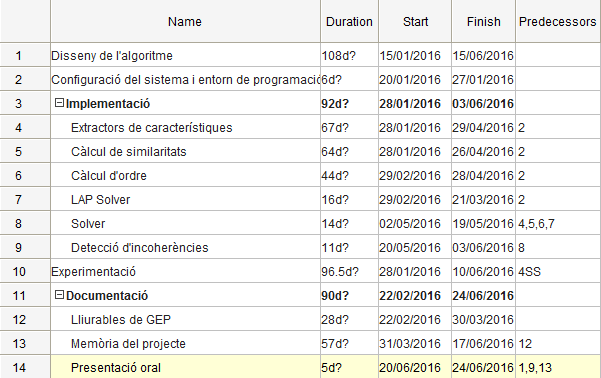
\includegraphics[width=\textwidth]{gantt1.png}
    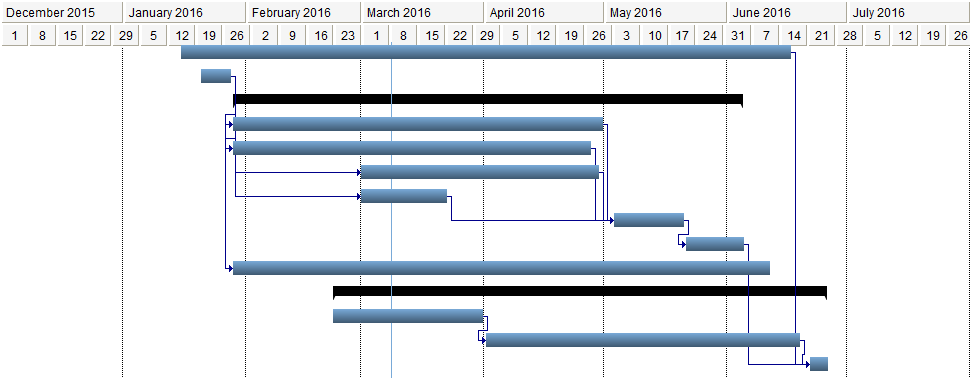
\includegraphics[width=\textwidth]{gantt2.png}
    \caption{El diagrama de gantt de la planificació temporal del projecte.}
    \label{fig:gantt}
\end{figure}

\subsection{Anàlisi d'alternatives i decisions}
\label{alternatives}

La idea inicial és dur a terme les tasques planejades tal com estan especificades al diagrama de Gantt de la figura \ref{fig:gantt}. No obstant això, s'ha de tenir en compte que aquest és un projecte amb un fort component exploratori. És per això que pot resultar difícil adaptar-se al pla dissenyat. Una decisió de disseny provinent de nous fets que surten fruit de l'experimentació pot fer que algun dels mòduls de l'algoritme deixi de ser necessari o necessiti canvis substancials. En aquest apartat es valoren les diferents alternatives plantejades en tots els apartats del projecte i es justifica, si escau, la alternativa escollida finalment.

El primer apartat on s'han plantejat diverses alternatives és en la quantitat de característiques a extreure del text i el model. Com més tipus de característiques s'explorin més qualitat tindrà l'algoritme\footnote{Aixo no vol dir que l'algoritme final faci l'extracció de totes les característiques implementades. Ans al contrari, com més d'aquestes es plantegin i s'avaluin més informat serà l'algoritme i per tant, en general, millor.}. En vista de resultats fruit de l'experimentació s'ha decidit optar per un conjunt relativament petit de característiques, ja que en la majoria de casos el subjecte d'una frase, o simplement l'aparició d'una paraula concreta, són suficients per a relacionar un fragment del text amb la tasca corresponent.

Un altre lloc on es troba una gran flexibilitat és en la quantitat d'experimentació. Com més alternatives s'exploren quant a mètriques de similaritat i algoritmes d'optimització millor serà l'algoritme final. En aquest cas, la majoria de tasques d'implementació han donat bastant bons resultats inicialment, així que no s'ha plantejat una experimentació molt profunda. On sí que s'està invertint una bona quantitat de temps és en la tasca actual: Escollir un solver per resoldre el problema de trobar una correspondència entre tasques i frases. Això és així perquè els primers intents de modelar del problema com una satisfacció de restriccions no han estat suficientment ràpids en temps d'execució.

Pel que fa a reduir el problema a un LAP, finalment s'ha optat --després d'experimentar-- per desestimar-ho. El valor d'ajustar el problema com un LAP no és més gran que el de utilitzar una altra solució inicial més simple.

Finalment, les alternatives pel que fa a la detecció d'inconsistències encara s'han de plantejar. De moment s'ha descartat la idea inicial, ja que l'enfoc proposat a \ref{el_paper} no és viable per a aquest projecte.

Com es pot veure a la taula de temps. La quantitat d'hores prevista per completar aquest projecte és de 540 hores. Tenint en compte que aquest projecte durarà 24 setmanes aproximadament, podem veure que surten 22,5 hores per setmana, que descomptant dos dies per setmana equival a 4,5 hores de treball diàries de mitjana. És viable dedicar aquesta quantitat de temps per a finalitzar el projecte en el període establert. 

De moment, tenint en compte els temps de treball diaris calculats es pot veure com la mitjana d'hores diàries és una mica inferior al valor calculat. Unes 4 hores de treball diari. No obstant si ens fixem en l'estat del projecte en la planificació a l'apartat \ref{estat}, veiem com la planificació avança segons el previst. Cal tenir en compte, però, que no és l'únic factor en joc: El cost del projecte recau principalment en les hores invertides. Per tant, és important contemplar aquesta estimació de cara al pressupost del projecte. En aquest cas, s'està parlant d'una lleugera desviació, d'aproximadament 30min per dia de mitjana, el que equivaldria a unes 60 hores. Cal estudiar si hi ha hagut una sobreestimació d'hores o si simplement aquestes hores seràn necessaries més endavant quedant concentrades a la part final del projecte.

\subsection{Estat del projecte en la planificació}
\label{estat}

El projecte es troba actualment en fase de desenvolupament. Aquest apartat descriu l'estat de cadascuna de les tasques plantejades a l'apartat \ref{descripcio_tasques}

Pel que fa al disseny de l'algoritme, aquest es troba en una fase avançada. Pràcticament s'han fixat ja la majoria de punts a decidir. Només queda planificar com serà el joc de proves per avaluar l'algoritme i decidir com s'avaluaràn les inconsistències. Finalment, el punt més important que queda per decidir és quin solver utilitzar per a calcular la correspondència entre tasques i frases.

Respecte la configuració de l'entorn de programació, aquesta està totalment finalitzada. La tasca es va realitzar abans de començar l'implementació en les hores establertes.

L'implementació de l'algoritme avança segons el previst. Actualment les tasques d'Extracció de característiques, càlcul de similaritat i càlcul d'ordre estàn acabades. Respecte el modelat del problema com un LAP, després d'implementar-ne una versió bàsica i realitzar diversos experimentar, es va desestimar i la tasca no s'ha arribat a finalitzar. Actualment, s'està treballant en modelar el problema amb un solver de satisfacció de restriccions. Finalment, encara s'ha de començar la tasca de detecció d'incoherències. 

Pel que fa a la tasca d'experimentació aquesta es duu a terme mentre durin l'implementació i el disseny. Els diferents experiments realitzats fins al moment han sigut molt útils per a determinar quines són les alternatives més viables per a resoldre els diversos obstacles que s'han trobat amb el projecte. El gruix d'aquesta tasca s'està duent a terme actualment, ja que s'està experimentant amb diferents tipus de models i solvers buscant una alternativa que pugui resoldre el problema amb un temps suficientment ràpid.

Finament, pel que fa la documentació, ja s'està elaborant la memòria final del projecte, segons l'establert a la planificació.

Com es pot veure, la planificació avança segons l'establert al diagrama de Gantt. Aquest document s'ha redactat el 10 de Maig de 2016 i l'estat del projecte és aproximadament l'esperat.

\clearpage

\section{Pressupost i sostenibilitat}

\subsection{Pressupost}
\label{pressupost}

En aquesta secció es fa un anàlisi detallat dels costos per a la realització d'aquest TFG. Els diferents apartats corresponen als diferents tipus de despeses que es plantegen. 

Cal tenir en compte que aquest pressupost s'ha dissenyat com si es tractés d'un projecte d'enginyeria en una empresa real, i que no tots els costos --Especialment els referents als recursos humans-- reflecteixen la realitat del projecte.

\subsubsection{Recursos humans}

La major part de tasques d'aquest projecte corresponen a una sola persona\footnote{Tret de la tasca de disseny de l'algoritme, que es realitza de manera conjunta entre l'alumne i els directors de projecte.}. Aquest, però, no seria el cas en un projecte real. A l'hora de fer aquest pressupost s'han tingut en compte els diferents rols que intervindrien en un projecte similar. Així doncs, els recursos humans s'han dividit en els rols de: Cap de projecte, dissenyador, programador, \emph{beta tester} i documentador.

Tenint en compte les diferents tasques definides a la planificació temporal, podem estimar les hores de cadascun dels membres de l'equip:

\begin{itemize}
    \item La configuració de l'entorn de programació correspondria al programador, que és qui estableix els requisits de l'entorn. (15h)
    \item El disseny de l'algoritme correspondria conjuntament al Cap de projecte i al Dissenyador. El temps planejat de la part de disseny no es parteix, és simultani\footnote{És important notar aquest fet, ja que fa que les hores del pressupost no sumin el mateix que les hores totals del projecte.}. (90+90h)
    \item La implementació de l'algoritme corresponen al programador i al \emph{beta tester}. El temps total es reparteix entre els dos rols. (180+70h)
    \item L'experimentació correspon al dissenyador, encarregat de dissenyar els experiments. Es comptabilitzen també unes hores del programador per implementar el codi dels experiments. (75+10h)
    \item La documentació correspon al rol de documentador. (100h)
\end{itemize}

A la taula \ref{tab:recursos_humans} es pot veure el pressupost estimat considerant un sou adequat per cadascun dels rols.

\begin{table}[!htb]
    \centering
    \begin{tabular}{|l||c|r|r|}
        \hline
         Rol & Preu per hora & Hores & Cost \\
         \hline\hline
         Cap de projecte & 50.00€/h & 90h & 4500.00€ \\
         Dissenyador & 35.00€/h & 165h & 5775.00€ \\
         Programador & 30.00€/h & 190h & 5700.00€ \\
         \emph{Beta tester} & 30.00€/h & 70h & 2100.00€ \\
         Documentador & 30.00€/h & 100h & 3000.00€ \\
         \hline\hline
         TOTAL & & & 21075.00€ \\
         \hline
    \end{tabular}
    \caption{Estimació del pressupost dels recursos humans.}
    \label{tab:recursos_humans}
\end{table}

\subsubsection{Recursos de hardware}

A la taula \ref{tab:recursos_hardware} es descriu el pressupost que s'ha estimat per als recursos de hardware necessaris per dur a terme el projecte. La falta de dades sobre les màquines del \emph{Textserver} fa que no en puguem estimar un pressupost. D'altra banda res impedeix instal·lar \emph{Freeling} en local i executar-lo en la mateixa màquina amb la qual es desenvolupa el projecte si el servidor suposa un cost important.

\begin{table}[]
    \centering
    \begin{tabular}{|l||r|c|r|}
        \hline
         Producte & Preu & Vida útil & Amortització \\
         \hline\hline
         Ordinador portàtil & 700.00€ & 4 anys & 50.00€ \\
         Màquines del \emph{Textserver} & 0.00€ & desconegut & 0.00€ \\
         \hline\hline
         TOTAL & 700.00€ & & 50.00€ \\
         \hline
    \end{tabular}
    \caption{Estimació del pressupost dels recursos de software.}
    \label{tab:recursos_hardware}
\end{table}


\subsubsection{Recursos de software}

A la taula \ref{tab:recursos_software} es descriu el pressupost estimat per als recursos de software del projecte. Com es pot observar el pressupost és purament un formalisme, ja que tots els recursos de software utilitzats són totalment gratuïts.

\begin{table}[!htb]
    \centering
    \begin{tabular}{|l||c|c|r|}
        \hline
         Producte & Preu & Vida útil & Amortització \\
         \hline\hline
         Freeling & 0.00€ & -- & 0.00€ \\
         Activiti & 0.00€ & -- & 0.00€ \\
         Arch GNU/Linux & 0.00€ & -- & 0.00€ \\
         Clojure & 0.00€ & -- & 0.00€ \\
         Java & 0.00€ & -- & 0.00€ \\
         Maven & 0.00€ & -- & 0.00€ \\
         \LaTeX & 0.00€ & -- & 0.00€ \\
         Gannter & 0.00€ & -- & 0.00€ \\
         \hline\hline
         TOTAL & & & 0.00€ \\
         \hline
    \end{tabular}
    \caption{Estimació del pressupost dels recursos de software.}
    \label{tab:recursos_software}
\end{table}


\subsubsection{Despeses indirectes}

Les despeses indirectes tenen en compte l'ús d'electricitat i material d'oficina necessaris per a la realització d'aquest projecte. La taula \ref{tab:recursos_indirectes} mostra una estimació del pressupost d'aquestes despeses.

El preu de l'electricitat s'ha calculat tenint en compte el preu del $KW/h$ a la ciutat de Barcelona i les hores del projecte en les que, segons la planificació, és necessari l'ús de l'ordinador\footnote{L'ordinador consumeix 120W, com es comenta a l'apartat de recursos.}. A més, s'inclou una part addicional en previsió de la llum necessària per desenvolupar el projecte.

Pel que fa al material d'oficina s'ha escollit un preu raonable per tal que la falta de material no resulti un inconvenient. Cal destacar que aquest projecte no en requereix un ús intensiu.

\begin{table}[!htb]
    \centering
    \begin{tabular}{|l||c|c|r|}
        \hline
         Producte & Preu & Unitats & Cost \\
         \hline\hline
         Electricitat (portatil) & 0.141€/KWh & 54Kwh\footnote{Connectat a la corrent sense bateria amb un transformador de 19V i 6.32A (120W).} & 7.61€\\
         \hline\hline
         Electricitat (llum) & 0.141€/KWh & 20Kwh\footnote{Dues bombetes de baix consum (15W)} & 7.61€\\
         \hline\hline
         Material d'oficina & 25.00€/unitat & 1 & 25.00€ \\
         \hline\hline
         TOTAL & & & 32.61€ \\
         \hline
    \end{tabular}
    \caption{Estimació del pressupost dels recursos indirectes.}
    \label{tab:recursos_indirectes}
\end{table}


\subsubsection{Pressupost total}

A la taula \ref{tab:total} es mostra el pressupost global del projecte, on es pot veure que la part que aporta més al cost del projecte és la dels recursos humans. A l'apartat \ref{economica} es realitza la valoració global d'aquest pressupost.

\begin{table}[!htb]
    \centering
    \begin{tabular}{|l|r|}
        \hline
         Concepte & Preu \\
         \hline\hline
         Recursos Humans & 21075.00€ \\
         Recursos de Software & 0.00€ \\
         Recursos de Hardware & 50.00€ \\
         Despeses indirectes & 32.61€ \\
         \hline\hline
         TOTAL & 21157.61€ \\
         \hline
    \end{tabular}
    \caption{Estimació del pressupost total.}
    \label{tab:total}
\end{table}

\subsection{Control de gestió}
\label{control}

En aquesta secció es considera com podria modificar-se aquest pressupost davant d'imprevistos i es proposen alternatives per tal de compensar-ho.

Com es veu a l'apartat anterior, pràcticament la totalitat del cost del projecte correspon als recursos humans. És per aquest fet que possibles desviacions en la planificació temporal poden afectar molt significativament al pressupost del projecte. Si es dóna el cas, cal sospesar si és més profitós reduir funcionalitats del projecte final o augmentar les hores totals del projecte. El primer escenari possiblement comportarà menys beneficis donat que s'haurà obtingut un producte de menys qualitat, mentre que amb el segon pot augmentar considerablement el pressupost final.

Pel que fa al software, un possible imprevist seria la incorporació de codi amb llicències de pagament en el projecte. En cas de ser inevitable s'haurà d'assumir el cost però sempre que sigui possible s'optarà per alternatives gratuïtes i, si és possible, de codi obert.

Pel que fa al hardware i al consum elèctric no es preveuen desviacions. Realment l'únic necessari per implementar l'algoritme és un ordinador i algun material complementari (papers, bolígrafs, etc.).

\subsection{Anàlisi de sostenibilitat}

En aquesta secció es descriu l'anàlisi de sostenibilitat feta per aquest projecte. En primer lloc es presenta la matriu de sostenibilitat del projecte i posteriorment se'n realitza una anàlisi per files justificant les puntuacions assignades a cada casella de la matriu.

\subsubsection{Matriu de sostenibilitat}
La taula \ref{tab:matriu_sostenibilitat} mostra la matriu de sostenibilitat d'aquest projecte. La puntuació de sostenibilitat total del projecte és de 70 punts, el que ens indica que és un projecte suficientment viable i sostenible.
\begin{table}[!htb]
    \centering
    \begin{tabular}{|c|c|c|c|}
    \hline
         & PPP & Vida útil & Riscos \\
         \hline\hline
        Ambiental & 10 & 19 & 0 \\
        \hline
        Econòmic & 8 & 15 & -12 \\
        \hline
        Social & 10 & 8 & -5 \\
        \hline\hline
        Puntuació & 28 & 42  & -17\\
        \hline
        \textbf{Total} & \multicolumn{3}{c|}{70} \\
        \hline
    \end{tabular}
    \caption{Matriu de sostenibilitat}
    \label{tab:matriu_sostenibilitat}
\end{table}

\subsubsection{Dimensió ambiental}

Aquest projecte no requereix l'ús de manera directa de cap agent contaminant. L'únic necessari per al desenvolupament de l'algoritme és un ordinador, i el producte final és software. Tot i això l'ús d'energia elèctrica i aparells electrònics comporta, indirectament, l'emissió de gasos contaminants a l'atmosfera. Fent una estimació\footnote{S'ha utilitzat la calculadora d'emissions de CO2 disponible a: \url{http://arboliza.es/compensar-co2/calculo-co2.html}} del $CO_2$ emès, es calcula que el desenvolupament d'aquest projecte comportarà l'emissió de 48.1Kg de $CO_2$ alliberats a l'atmosfera. És important destacar que la utilització d'un ordinador portàtil com a eina principal de desenvolupament fa que el consum energètic sigui considerablement inferior que si s'hagués utilitzat un ordinador de sobretaula\footnote{Un ordinador de sobretaula equivalent consumiria uns 400W de mitjana en comptes dels 120W que gasta el portàtil.}. En tot cas, la quantitat de $CO_2$ generada per aquest projecte és molt inferior a la que genera una persona en els 6 mesos de durada d'aquest. Per aquest fet, s'ha donat la puntuació màxima de 10 punts a la casella Ambiental/PPP de la matriu.

Si aquest projecte s'acaba convertint en un software exitós, és probable que moltes empreses l'incorporin en els seus servidors i l'utilitzin de manera extensiva. És difícil estimar el consum energètic que això comportarà, però és innegable que un software executant-se contínuament en els servidors d'una empresa i que fa servir algoritmes costosos té un cost energètic no negligible. D'altra banda, aquest fet es veuria possiblement compensat per l'estalvi de paper i material que suposaria l'automatització de totes les tasques relacionades amb el \emph{Business Process Management}. És per aquest fet que s'ha donat una puntuació de 19 a la casella Ambiental/Vida útil de la matriu de sostenibilitat. 

Finalment, cal comentar que no es preveu cap escenari en el qual aquest projecte pugui augmentar la seva petjada ecològica més enllà del que ja s'ha comentat en aquest document. És per això que s'assigna una puntuació de 0 a la casella Ambiental/Riscos.


\subsubsection{Dimensió econòmica}
\label{economica}

A l'apartat \ref{pressupost} ja es realitza una anàlisi detallat de tots els costos que intervenen en aquest projecte, tant humans com materials. Cal tenir en compte, però, que aquest és le pressupost de realització del projecte l'objectiu del qual és crear un software. El software resultant molt probablement requereixi manteniment, actualitzacions i expansions. 

És difícil reduir costos durant la realització del projecte. Quasi tot el cost del projecte recau en el cost dels sous dels desenvolupadors i les hores vénen marcades per la planificació temporal. No obstant una planificació més compacta i no tan centrada en l'experimentació podria ajudar a millorar en l'àmbit econòmic. El fet que aquest projecte aborda un problema que gairebé no s'ha tractat fins al moment a la literatura fa que sigui molt difícil parlar de reaprofitar codi per l'algoritme. A part, el cost tant en software com hardware és el mínim necessari. Per tot això s'assigna una puntuació de 8 a la casella Econòmic/PPP.

L'objectiu del projecte global és comercialitzar el producte resultant a empreses\footnote{Cal recordar que l'objectiu d'aquest TFG és l'algoritme que es desenvolupa en aquest TFG passi a formar part d'un paquet software que pugui servir per a les empreses centrades en \emph{Business Process Management}. Em refereixo a això amb el projecte global.}. La viabilitat econòmica d'aquest paquet de software depèn del model de distribució que s'esculli per comercialitzar-lo. Per una banda es pot optar per una llicència tancada i de pagament. Una possible alternativa a la venda per llicència, és un model de doble llicència: S'ofereix una versió bàsica del producte com a software gratuït perquè qualsevol empresa el pugui provar i es cobra per la versió completa, que permet l'ús del software per a mitjans comercials. És difícil determinar a priori el potencial de vendes del producte resultant, però si l'algoritme genera bons resultats, pot arribar a ser una eina de gran valor per a empreses centrades en el BPM. És per això que s'ha donat una puntuació de 16 a la casella Econòmic/Vida útil.

Si l'enfoc del tractament automàtic del \emph{Business Process Management} resulta profitós a les empreses centrades en aquesta pràctica, és molt probable que apareguin tot tipus de competidors al software d'aquest projecte. No obstant cal tenir en compte que s'estaria partint d'una posició avantatjosa, ja que aquest seria el primer software al mercat a oferir funcionalitats similars. És doncs important tenir en compte aquest risc a l'hora de comercialitzar el software final i per això s'ha donat una puntuació de -12 a la casella Econòmic/Riscos.

\subsubsection{Dimensió social}

Aquesta és, potser, la dimensió més rellevant per aquest projecte. Tant en aspectes positius com també en negatius.

Pels actors implicats en el desenvolupament d'aquest projecte, el desenvolupament d'aquest comporta un creixement personal. Concretament, com a alumne, m'acosta al món de la recerca, i em dóna una bona visió de l'algorítmia en un entorn pràctic i realista com és el \emph{Business Process Management} en combinació amb el \emph{Natural Language Processing}. A part, el fort component de programació del projecte i l'elecció de les eines de treball em comporta un creixement personal especialment com a programador. A més d'haver treballat en un projecte gran i amb utilitat pràctica directa per primera vegada. És per això que he puntuat amb un 10 la casella Social/PPP de la matriu.

La documentació i anàlisi dels processos de negoci en empreses resulta una manera molt bona de controlar les activitats d'una empresa de cara a optimitzar-ne el cost. És evident, doncs, que l'automatització d'aquestes tasques tindrà un impacte positiu directe en el rendiment econòmic de l'empresa. A més, l'algoritme desenvolupat en aquest TFG pot estalviar una gran quantitat d'hores de treball repetitiu assistint en la cerca d'incoherències entre els models BPMN i les seves representacions textuals. No obstant això, aquest mateix estalvi pot resultar en un impacte negatiu pel col·lectiu d'empleats que treballi desenvolupant aquestes mateixes tasques. Aquest últim fet es veuria especialment accentuat si les empreses decideixen retallar en la seva plantilla com a resultat de l'automatització d'aquesta tasca. És per això que s'assigna una puntuació de 15 a la casella Social/Vida útil de la matriu de sostenibilitat.

Com ja s'ha comentat, la pèrdua de llocs de treball fruit de l'automatització de les tasques en les quals assisteix l'algoritme d'aquest projecte pot ser vista com un risc per a la gent que treballa en aquest tipus de feines. No obstant s'ha de tenir en compte que això també pot ser vist com una oportunitat de reassignar aquests treballadors en tasques de més alt nivell. A més, si el resultat d'aquest projecte comporta beneficis a una empresa aquesta té un major potencial de creació de llocs de treball. Hi han riscos, però es poden evitar. Per això s'assigna una puntuació de -5 a la casella Social/Riscos de la matriu de sostenibilitat.

\section{Integració de coneixements}
\label{integracio}
En aquesta secció es discuteixen les diferents disciplines de la informàtica que intervenen en aquest projecte en més o menys mesura i com hi estàn integrades.

Aquest projecte és una combinació de dues disciplines concretes de la informàtica. El \textit{Natural Language Processing} i el \textit{Business Process Management}. Els dos camps es troben en recerca activa i els resultats obtinguts en aquests utilitzen tot tipus de tècniques de diferents camps com la intel·ligència artificial, la teoria de grafs o l'algorísmia.

Per a l'elaboració del projecte s'utilitzen, o s'han plantejat utilitzar\footnote{No totes les alternatives plantejades han acabat al projecte original, però això no vol dir que no s'hagin estudiat i valorat.} les següents tècniques i algoritmes relacionades amb els continguts de la carrera:

\begin{itemize}
\item Freeling, com a analitzador semàntic.
\item Solver de Constraint Programming.
\item Mètriques de distancia.
\item Vectors de característiques.
\item Similaritat semàntica en Wordnet.
\item Càlcul de Behavioral Profiles en grafs de processos.
\item Algoritmes de grafs de flux, concretament el d'eliminació de back-edges.
\item Linear Assignment Problem i l'Hungarian Method.
\item Programació funcional.
\end{itemize}

\section{Lleis i regulacions}
\label{lleis}
En aquest apartat es fa una breu discussió de l'apartat legal rellevant en el marc del projecte.

Pel que fa al producte resultant, aquest és una eina que està planejada per assistir en tècniques de Business Process Management. Actualment no existeix cap legislació que reguli com una empresa ha de documentar els seus processos des d'un punt de vista de BPM, i si es requerís d'alguna documentació en un camp concret aquesta existeix separada de la documentació formal dels processos de negoci. Així doncs podem dir que no hi ha cap normativa que s'hagi de tenir en compte a l'hora de parlar del producte resultant.

No obstant, pel que fa al desenvolupament del software i les opcions de comercialització, cal tenir en compte quines són les llicències utilitzades en totes les llibreries que aquest integra, i quina serà la llicència del producte final. S'ha d'anar en compte amb no incumplir cap dels termes i condicions de totes les llicències que s'estàn fent servir. 

\printbibliography[heading=bibliography]{}
\end{document}
